\documentclass{article}
\usepackage{graphicx} % Required for inserting images
\usepackage{amsmath}
\usepackage{amssymb}
\usepackage{float}
\usepackage{textgreek}
\usepackage{fancyhdr}
\usepackage{hyperref}
\usepackage{tikz}
\usetikzlibrary{shapes,arrows}
\usepackage{enumerate}

% vnořené popisky obrázků
\usepackage{subcaption}

% automatická konverze EPS 
\usepackage{graphicx} 
\usepackage{epstopdf}

\pagestyle{fancy}
\newcommand\mat[1]{\begin{bmatrix}#1\end{bmatrix}}

\title{ARI-HW\_08}
\author{Matěj Pinkas}
\date{14. April 2024}

\lhead{Pinkas Matěj}
\chead{ARI-HW\_08}
\rhead{14. April 2024}


\begin{document}

\maketitlessz

\section{Příklad: Model HIV - AIDS}
\begin{itemize}
    \item[-] Zadání: 
    \begin{align*}
        \mat{\dot{T}\\\dot{T}^*\\\dot{v}} &= \mat{-0,04167 & 0 & -0,0058\\0,0217 & -0,24 & 0,0058\\0 & 100 & -2,4} = \mat{T\\T^*\\v} + \mat{5,2\\-5,2\\0}u_1\\
        y &= \mat{0 & 0 & 1} \mat{T\\T^*\\v}
    \end{align*}
    \item[] $T$ je počet zdravých buněk, $T^*$ je počet infikovaných buňek a $v$ je počet volných částic viru v krvi pacienta
    \item[] Vstupem systému je dávkování $u_1 \in [0,1]$ a výstupem je počet částic viru
    
    \item[-] Ze zadání vytvořím z modelu stavové matice A, B, C, D:

    \begin{align*}
        A &= \mat{-0,04167 & 0 & -0,0058\\
                 0,0217 & -0,24 & 0,0058\\
                 0 & 100 & -2,4} 
        & 
        B &= \mat{5,2\\ -5,2\\ 0}\\
        C &= \mat{0 & 0 & 1}
        &
        D &= \mat{0}
    \end{align*}

    \item[-] Spočítám si přenos tohoto systému:
    \begin{align*}
        G(s) = \mathbf{C}(s\mathbf{I}-\mathbf{A})^{-1}\mathbf{B}+\mathbf{D} = \frac{-520s-10,38}{s^3+2,682s^2+0,106s+0,01242}\\
        zero(G(s)) = -0,02
    \end{align*}

    \item[-] Z dalších zadaných hodnot $OS_\%$ a $T_s$ spočítám relativní tlumení a přirozenou frekvenci:
    \begin{align*}
        OS_\% &= 10\% & OS &= 0,1 & T_s &= 100 \ \text{[dní]}
    \end{align*}
    
    \begin{align*}
        \zeta &= -\frac{\ln{(OS)}}{\sqrt{\pi^2+\ln{(OS)}^2}} \approx 0,591155\\
        \omega_n &= \frac{-\ln{\left(0,02\sqrt{1-\zeta^2}\right)}}{T_s\zeta} = 0,0698
    \end{align*}

    \item[-] Získám přenos z vypočtených hodnot:
    \begin{align*}
        H(s) = \frac{\omega_n^2}{s^2+2\zeta \omega_ns+\omega_n^2} = \frac{0,0048737}{s^2+0,082540s+0,0048737}
    \end{align*}
    \item[-] Z přenosu získám charakteristický polynom: 
    \begin{align*}
        c_H(s) = s^2 + 2\omega_n\zeta s+\omega_n^2 = s^2+0,082540s+0,0048737
    \end{align*}

    \item[-] Zavedení zpětné stavové vazby $\mathbf{K}$ a další integrační parametr $K_I$
    \begin{align*}
        \mathbf{K} = \mat{K_1 & K_2 & K_3}
    \end{align*}
    \item[-] Pro tyto konstanty vytvořím nové stavové matice z už stávajících A, B, C, D 
    \begin{align*}
        \mathbf{A}_N &= \mat{\mathbf{A}-\mathbf{BK} & \mathbf{B}K_I\\
                             -\mathbf{C} & 0} 
        & 
        \mathbf{B}_N &= \mat{0\\ 0\\ 0\\ 1}\\
        \mathbf{C}_N &= \mat{\mathbf{C} & 0} 
        &
        \mathbf{D}_N &= \mat{0}
    \end{align*}

    \item[-] Vypočtu si charakteristický polynom těchto nových stavových matic s parametry $K_1$, $K_2$, $K_3$ a $K_I$:
    \begin{align*}
        c_N(s) &= \det{(s\mathbf{I}-\mathbf{A}_N)} =\\
        &s^4 + s^3(5,2K_1-5,2K_2+2,68167) + s^2(13,728K_1-12,583844K_2-520K_3+0,1060088)+\\
        &s(2,9952K_1+0,01241932-520K_I-10,3844K_3-0,2492256K_2) -10,3844K_I
    \end{align*}

    \item[-] Charakteristický polynom $c_H(s)$ rozšířím o další 2 póly, abych vyrovnal řád polynomu $c_N$
    \item[-] Polynom rozšířím o pól v nule původního sytému, tedy v $-0,02$ a o druhý pól ve stabilní levé části co nejdále aby systém příliš neovlivnil, například $-100$
    \begin{align*}
        c_{HN}(s) &= (s^2+0,082540s+0,0048737)(s+0,02)(s+100) =\\ 
        &s^4+100,1s^3+10,26s^2+0,6525s+0,009747
    \end{align*}

    \item[-] Nyní stanovým polynomy $c_{N}$ a $c_{HN}$ sobě rovny, tím získám soustavu rovnic pro proměnné $K_1$, $K_2$. $K_3$, a $K_I$:
    \begin{align*}
        100,1 &= 5,2K_1-5,2K_2+2,68167\\
        10,26 &= 13,728K_1-12,583844K_2-520K_3+0,1060088\\
        0,6525 &= 2,9952K_1+0,01241932-520K_I-10,3844K_3-0,2492256K_2\\
        0,009747 &= -10,3844K_I
    \end{align*}
    \item[-] Po vyřešení soustavy rovnic získám: 
    \begin{align*}
        K_1 &= -0,0043795 &
        K_2 &= -18,738673 &
        K_3 &= 0,43382775 &
        K_I &= -0,0009386
    \end{align*}

    \item[-] Tyto získané konstatny dosadím do stavových matic $A_N$, $B_N$, $C_N$ a $D_N$
    \item[-] Z těchto matic spočítám přenos:
    \begin{align*}
        H_N(s) = \frac{0,4881s + 0,009747}{s^4+100,1s^3+10,26s^2+0,6525s+0,009747}
    \end{align*}

    \begin{figure}[H]
        \centering
        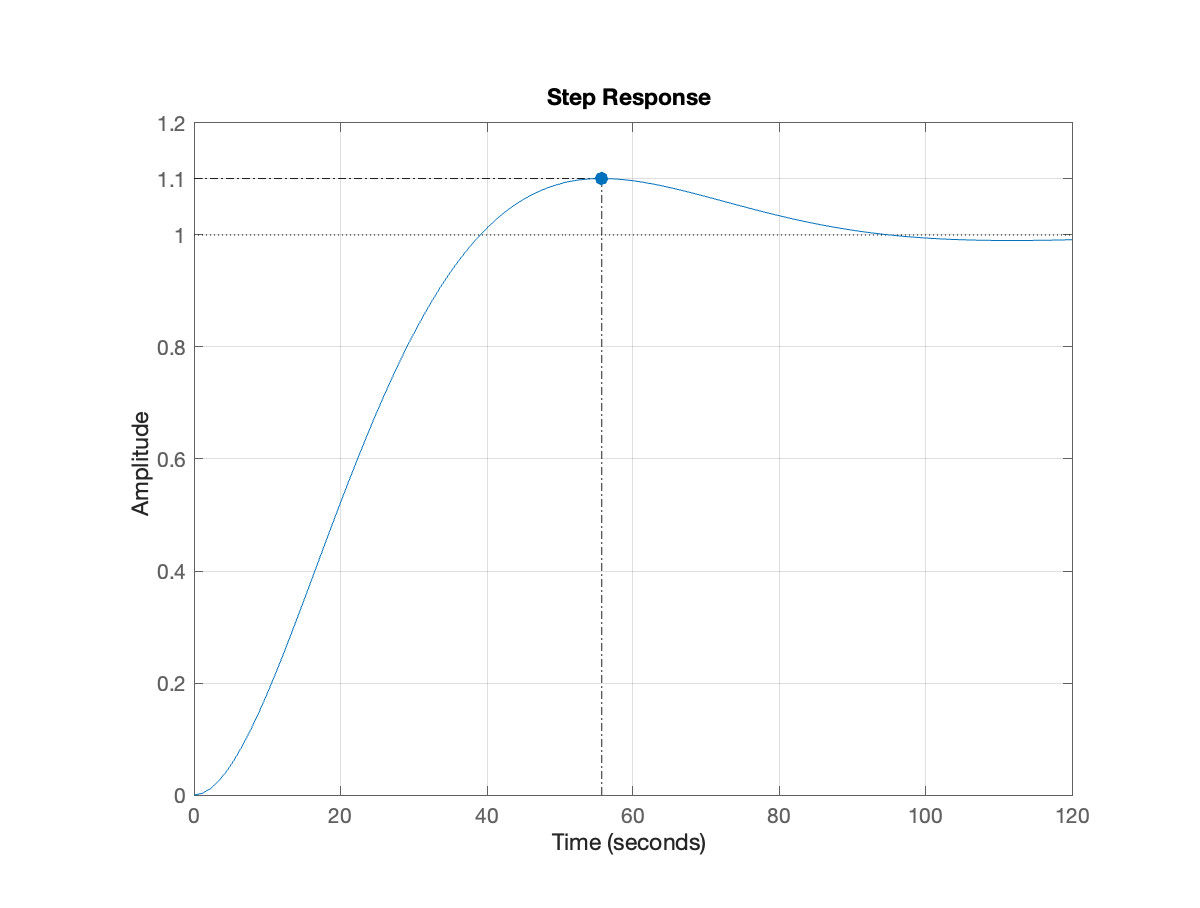
\includegraphics[clip, width=1.00\textwidth]{Step_response.eps}
        \caption{Odezva na jednotkový skok systému se stavovou zpětnou vazbou}
        \label{fig:Step_response}
    \end{figure}
    \item[-] Z grafu je vidět, že systém dodržuje zadané parametry, maximální překmit $10\%$ a dobu ustálení do 100 dní
\end{itemize}

\end{document}
